La struttura di base del programma è stata sviluppata in ottica modulare 
utilizzando il linguaggio C++ e la sua libreria standard: a 
run-time è possibile specificare plug-in diversi per gestire la logica dei 
Robby. Tali plug-in devono implementare diverse funzioni: muovere il Robby 
scegliendo la direzione appropriata, generare le strutture dati proprie 
all'algoritmo (es. le reti neurali o i genomi per l'algoritmo genetico puro) e 
liberare la memoria allocata in precedenza. La logica di base del programma 
rimane invece invariata, compresa la funzione di fitness. Tale funzione 
deve tenere conto del numero di lattine raccolte e di eventuali fallimenti 
nelle mosse effettuate (se il Robby si muove nella direzione di un muro, 
oppure 
tenta di raccogliere una lattina su una cella vuota). La fitness è definita 
come segue:
\[\sum\limits_{i=0}^{r} \frac{gc_i}{tc\cdot mn+1}+\frac{sm_i}{t\cdot (tc 
\cdot mn + 1)}\]
Dove:
\begin{itemize}
 \item $r$ è il numero di Robby presenti su ciascuna mappa;
 \item $gc_i$ è il numero di lattine raccolte dall'i-esimo Robby;
 \item $tc$ è il numero totale di lattine per ciascuna mappa;
 \item $mn$ è il numero totale di mappe;
 \item $sm_i$ è il numero di mosse corrette effettuate dall'i-esimo Robby;
 \item $t$ è il numero di turni totali concessi al singolo Robby.
\end{itemize}
Tale formula considera il successo di tutte le mosse possibili come la raccolta 
di una singola lattina ed incrementa di uno il numero totale di lattine. Il 
valore della funzione è compreso fra 0 e 1, dove 0 è il fallimento totale, 
mentre 1 è il successo totale (tutte le lattine raccolte, nessuna mossa 
sbagliata).
\\
Al fine di consentire la comunicazione dei Robby, viene mantenuta una lista 
globale di messaggi. Ciascun messaggio contiene l'identificatore univoco del 
Robby mittente, la propria vista locale, la propria posizione e l'ultima mossa 
da esso effettuata. Tali informazioni vengono poi combinate dal plug-in 
selezionato per scegliere la strategia migliore.
\\
La vista locale ai Robby è una semplice matrice quadrata che viene popolata dal 
core del programma per mostrare ciò che vede il Robby entro una distanza 
specificata parametricamente. Tale vista non è però quadrata: alcune celle che 
sarebbero incluse in una vista quadrata sono più distanti dal Robby rispetto al 
raggio specificato. Per ovviare a tale problema si è scelto di procedere 
utilizzando il seno discreto per distinguere le celle visibili in questo modo:
\[height(n)=\lfloor r \cdot sin(n\cdot\frac{\pi}{2\cdot r})\rfloor \]
Dove:
\begin{itemize}
  \item $r$ è il raggio del cerchio da generare; 
  \item $n$ è il valore intero che rappresenta la distanza tra il punto in 
  esame sull'asse delle ascisse e il centro, ed è quindi compreso fra 1 e r.
\end{itemize}
Si procede iterando n per calcolare quante celle considerare sull'asse delle 
ordinate sopra alla cella individuata da n. Si ottiene così un quarto di 
cerchio, ed è quindi possibile ruotarlo per ottenere l'intero cerchio discreto.
Una volta ottenuto tale cerchio, le celle al suo interno vengono popolate con 
valori interi che ne rappresentano lo stato (vuoto, lattina, Robby). Le celle 
esterne che sono presenti sulla matrice quadrata vengono impostate come 
sconosciute e non sono considerate dall'algoritmo.
\\
Per implementare la vista globale (detta anche known map) prima di ciascun 
turno vengono controllate le viste locali dei Robby e vengono applicate sulla 
mappa globale le informazioni da esse ricavate. Si ottiene così una vista
globale della mappa nella quale le celle sono sconosciute, vuote o contenti
lattine.
\\

Rispetto all'approccio NEAT classico si sono rese necessarie alcune modifiche
per adattare la tecnica al problema in esame. Nell'articolo 
originale\cite{stanley2002evolving} le nuove reti
vengono inizializzate come completamente connesse. Nell'implementazione
presentata si è scelto di procedere con reti inizialmente vuote (prive di
archi) al fine di consentire la ricerca di una rete che abbia una struttura
minimale.\\

Rispetto all'evoluzione topologica, l'algoritmo NEAT genera reti che possono
contenere cicli. Tali reti, che vengono dette ricorrenti (\emph{recurrent neural
network}), offrono vantaggi espressivi soprattutto per problemi nei quali ci sia
la necessità di mantenere una ``memoria" all'interno della rete, che pertanto
non viene azzerata tra due esecuzioni. Tale struttura risulta molto adatta a
gestire un flusso continuo di dati. Tuttavia, rispetto al problema in esame,
tale topologia della rete non offre vantaggi significativi e introduce 
complessità
computazionale nell'attivazione della rete, che deve essere strutturata per
evitare l'occorrenza di cicli infiniti che farebbero altrimenti divergere
l'intero algoritmo. Per ovviare a tale problema si è esteso l'algoritmo NEAT per
impedire la creazione di cicli durante l'evoluzione della rete. A tal fine si è
associata a ciascun nodo una frazione, che indica il livello a cui il nodo
appartiene. Tali valori sono compresi tra 0 e 1 e vengono considerati durante
la \emph{mutazione delle connessioni} e la \emph{mutazione dei nodi}. Durante la
mutazione delle connessioni i livelli dei due nodi adiacenti all'arco da inserire
vengono controllati e, nel caso in cui la connessione sia orientata dal livello
più alto verso il più basso viene invertito il verso dell'arco. Nel caso in cui
i due nodi siano sullo stesso livello l'arco non viene aggiunto. Durante la
mutazione dei nodi il valore del nuovo neurone viene calcolato come la il valore
medio tra i due livelli fra cui verrà inserito (\cref{fig:mutatefraction}).
Tale approccio introduce un ordinamento totale fra livelli, impedendo la
creazione di cicli senza aumentare la complessità computazionale.

\begin{figure}
	\centering
	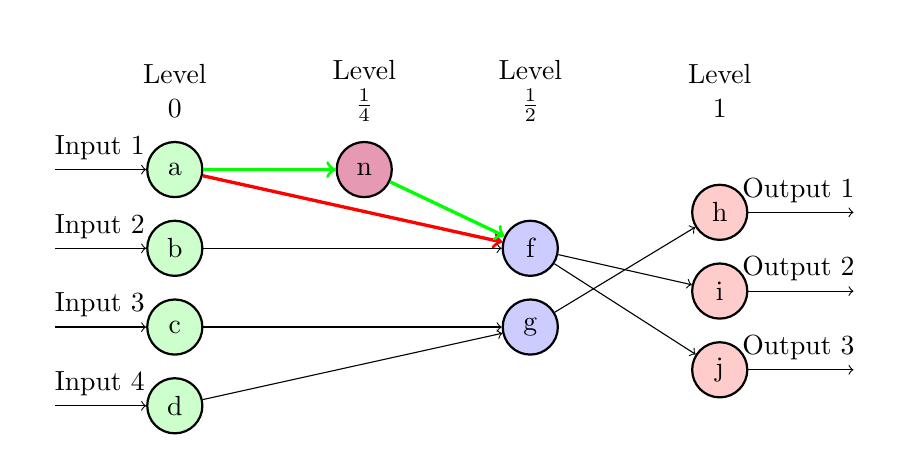
\begin{tikzpicture}[
		->,
		input node/.style={circle, draw, thick, fill=green!20,minimum size = 7mm},
		hidden node/.style={circle, draw, thick, fill=blue!20,minimum size = 7mm},
		output node/.style={circle, draw, thick, fill=red!20,minimum size = 7mm},
		new node/.style={circle, draw, thick, fill=purple!40,minimum size = 7mm},
		dummy node/.style={circle, thick}
	]
		\node[dummy node] (d1) {};
		\node[dummy node,below of=d1] (d2) {};
		\node[dummy node,below of=d2] (d3) {};
		\node[dummy node,below of=d3] (d4) {};

		\node[input node,right of=d1,xshift=20pt] (i1) {a};
		\node[input node,below of=i1] (i2) {b};
		\node[input node,below of=i2] (i3) {c};
		\node[input node,below of=i3] (i4) {d};

		\node[hidden node,right of=i2,xshift=100pt] (h1) {f};
		\node[hidden node,right of=i3,xshift=100pt] (h2) {g};

		\node[output node,right of=h1,yshift=13pt,xshift=40pt] (o1) {h};
		\node[output node,below of=o1] (o2) {i};
		\node[output node,below of=o2] (o3) {j};

		\node[dummy node,right of=o1, xshift=25pt] (do1) {};
		\node[dummy node,below of=do1] (do2) {};
		\node[dummy node,below of=do2] (do3) {};

		\foreach \i in {1,...,4} {
			\draw[<-] (i\i) -- (d\i) node[above,xshift=0.75cm] {Input \i};
		}

		\draw[->,very thick,red] (i1) -- (h1) {};
		\draw[->] (i2) -- (h1) {};
		\draw[->] (i3) -- (h2) {};
		\draw[->] (i4) -- (h2) {};

		\draw[->] (h1) -- (o3) {};
		\draw[->] (h1) -- (o2) {};
		\draw[->] (h2) -- (o1) {};

		\node[new node,right of=i1,xshift=40pt] (n1) {n};
		\draw[->,very thick,green] (i1) -- (n1) {};
		\draw[->,very thick,green] (n1) -- (h1) {};

		\foreach \o in {1,...,3} {
			\draw[<-] (do\o) -- (o\o) node[above,xshift=1cm] {Output \o};
		}

		\node[dummy node, above of=i1,text width=1cm, align=center]
		(lin) {Level 0};
		\node[dummy node, right of=lin,text width=1cm,align=center,
		xshift=40pt] (lhi) {Level $\frac{1}{4}$};
		\node[dummy node, right of=lin,text width=1cm,align=center,
		xshift=100pt] (lhi) {Level $\frac{1}{2}$};
		\node[dummy node, right of=lhi,text width=1cm,align=center,
		xshift=40pt] (lou) {Level 1};

		
	\end{tikzpicture}
	\caption{Mutazione di un nodo con il meccanismo delle frazioni. Dopo aver
	selezionato l'arco $(a,f)$ viene aggiunto il nodo $n$ e viene posizionato su
	un livello intermedio fra 0 e $\frac{1}{2}$. Il nuovo livello ha quindi
	valore $\frac{1}{4}$. Sono rappresentati in rosso l'arco disabilitato 
	e in verde i nuovi archi.}
	\label{fig:mutatefraction}
\end{figure}

\begin{figure}[H]
\begin{minipage}{.20\textwidth}
\begin{tikzpicture}[
		->,
		input node/.style={circle, draw, thick, fill=green!20,minimum size = 3mm},
		hidden node/.style={circle, draw, thick, fill=blue!20,minimum size = 3mm},
		output node/.style={circle, draw, thick, fill=red!20,minimum size = 3mm},
		dummy node/.style={circle, thick}
]
	\node[dummy node] (pi0) {};
	\node[input node, right of=pi0] (i0) {};
	\draw (pi0) -- (i0);

	\foreach \i in {1,...,5} {
		\auxcount=\i;
		\advance\auxcount by -1;
		\node[dummy node, below of=pi\the\auxcount](pi\i) {};
		\node[input node, below of=i\the\auxcount](i\i) {};

		\draw (pi\i) -- (i\i);
	}

	\node[output node,right of=i1,xshift=1cm] (o0) {};
	\node[dummy node,right of=o0] (po0) {};
	\draw (o0) -- (po0);
	\foreach \o in {1,...,3} {
		\auxcount=\o;
		\advance\auxcount by -1;
		\node[output node, below of=o\the\auxcount](o\o) {};
		\node[dummy node, below of=po\the\auxcount](po\o) {};
		\draw (o\o) -- (po\o);
	}
\end{tikzpicture}
\subcaption{}
\label{fig:mut1}
\end{minipage}
\hspace{.10\textwidth}
\begin{minipage}{.20\textwidth}
\begin{tikzpicture}[
		->,
		input node/.style={circle, draw, thick, fill=green!20,minimum size = 3mm},
		hidden node/.style={circle, draw, thick, fill=blue!20,minimum size = 3mm},
		output node/.style={circle, draw, thick, fill=red!20,minimum size = 3mm},
		dummy node/.style={circle, thick}
]
	\node[dummy node] (pi0) {};
	\node[input node, right of=pi0] (i0) {};
	\draw (pi0) -- (i0);

	\foreach \i in {1,...,5} {
		\auxcount=\i;
		\advance\auxcount by -1;
		\node[dummy node, below of=pi\the\auxcount](pi\i) {};
		\node[input node, below of=i\the\auxcount](i\i) {};

		\draw (pi\i) -- (i\i);
	}

	\node[output node,right of=i1,xshift=1cm] (o0) {};
	\node[dummy node,right of=o0] (po0) {};
	\draw (o0) -- (po0);
	\foreach \o in {1,...,3} {
		\auxcount=\o;
		\advance\auxcount by -1;
		\node[output node, below of=o\the\auxcount](o\o) {};
		\node[dummy node, below of=po\the\auxcount](po\o) {};
		\draw (o\o) -- (po\o);
	}

	\draw (i3) -- (o1);
\end{tikzpicture}
\subcaption{}
\label{fig:mut2}
\end{minipage}
\hspace{.10\textwidth}
\begin{minipage}{.20\textwidth}
\begin{tikzpicture}[
		->,
		input node/.style={circle, draw, thick, fill=green!20,minimum size = 3mm},
		hidden node/.style={circle, draw, thick, fill=blue!20,minimum size = 3mm},
		output node/.style={circle, draw, thick, fill=red!20,minimum size = 3mm},
		dummy node/.style={circle, thick}
]
	\node[dummy node] (pi0) {};
	\node[input node, right of=pi0] (i0) {};
	\draw (pi0) -- (i0);

	\foreach \i in {1,...,5} {
		\auxcount=\i;
		\advance\auxcount by -1;
		\node[dummy node, below of=pi\the\auxcount](pi\i) {};
		\node[input node, below of=i\the\auxcount](i\i) {};

		\draw (pi\i) -- (i\i);
	}

	\node[hidden node,right of=i3,yshift=.5cm] (h0) {};

	\node[output node,right of=i1,xshift=1cm] (o0) {};
	\node[dummy node,right of=o0] (po0) {};
	\draw (o0) -- (po0);
	\foreach \o in {1,...,3} {
		\auxcount=\o;
		\advance\auxcount by -1;
		\node[output node, below of=o\the\auxcount](o\o) {};
		\node[dummy node, below of=po\the\auxcount](po\o) {};
		\draw (o\o) -- (po\o);
	}

	\draw (i3) -- (h0);
	\draw (h0) -- (o1);
\end{tikzpicture}
\subcaption{}
\label{fig:mut3}
\end{minipage}
\caption{Un'evoluzione di esempio di una rete: La rete è inizialmente vuota
(\cref{fig:mut1}),
per poi mutare (tramite una \textbf{mutazione delle connessioni}) un arco tra
due nodi scelti casualmente
(\cref{fig:mut2}),
infine avviene una \textbf{mutazione di nodo} sul
collegamento appena creato
(\cref{fig:mut3})
.}
\centering
\end{figure}
